\subsection{Simulation Study}
To validate the variational model, we conduct a simulation study.
    As we are interested in an angular model, the data is generated from 
    a finite mixture of projected gammas distribution, at varying levels
    of dimensionality and number of mixture components.  For each simulation,
    1000 replicates are sampled.



In Figure~\ref{fig:energyscore} we compare the rise in energy score of the fitted
    model over a baseline energy score.


\begin{figure}[ht]
    \caption{Rise in energy score over baseline (Y) versus dimensionality (X), 
            by number of latent mixture components in generating distribution
            \label{fig:energyscore}}
    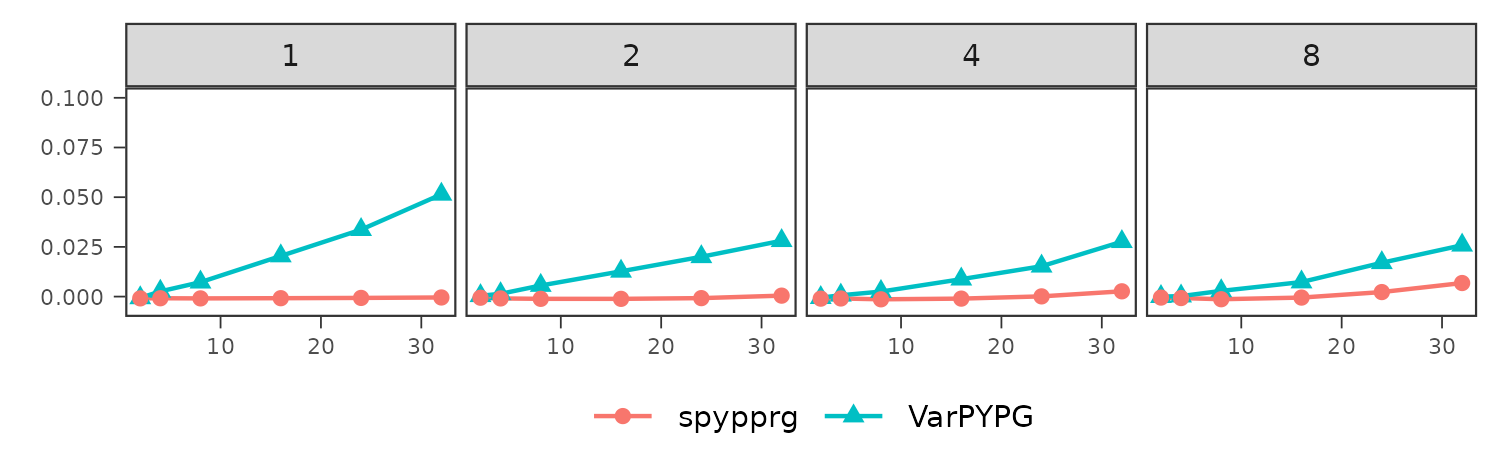
\includegraphics{./plots/energy_score}
\end{figure}


% EOF